% Para utilizar este template siga o tutorial disponível em http://www.biblioteca.ufc.br/wp-content/uploads/2015/09/tutorial-sharelatex.pdf

\documentclass[        
    a4paper,          % Tamanho da folha A4
    12pt,             % Tamanho da fonte 12pt
    chapter=TITLE,    % Todos os capitulos devem ter caixa alta
    section=Title,    % Todas as secoes devem ter caixa alta somente na primeira letra
    subsection=Title, % Todas as subsecoes devem ter caixa alta somente na primeira letra
    oneside,          % Usada para impressao em apenas uma face do papel
    english,          % Hifenizacoes em ingles
    spanish,          % Hifenizacoes em espanhol
    brazil,           % Ultimo idioma eh o idioma padrao do documento
    fleqn             % Comente esta linha se quiser centralizar as equacoes. Comente também a linha 65 abaixo
]{abntex2}


\input{lib/preambulo}

\setlength{\mathindent}{0pt} %Complementa o alinhamento de equações para totalmente a esquerda.

%%%%%%%%%%%%%%%%%%%%%%%%%%%%%%%%%%%%%%%%%%%%%%%%%%%%%
%%                     ATENCAO                     %%
%%%%%%%%%%%%%%%%%%%%%%%%%%%%%%%%%%%%%%%%%%%%%%%%%%%%%
%  Qual e o nivel do trabalho academico que voce esta 
% escrevendo? Retire o simbolo "%" apenas de um dos 
% quatro topicos abaixo refente ao nível do seu traba
% -lho.

%\trabalhoacademico{tccgraduacao}
%\trabalhoacademico{tccespecializacao}
\trabalhoacademico{dissertacao}
%\trabalhoacademico{tese}

%%%%%%%%%%%%%%%%%%%%%%%%%%%%%%%%%%%%%%%%%%%%%%%%%%%%%

% Define se o trabalho e uma qualificacao
% Coloque 'nao' para versao final do trabalho

\ehqualificacao{nao}

% Remove as bordas vermelhas e verdes do PDF gerado
% Coloque 'sim' pare remover

\removerbordasdohyperlink{sim} 

% Adiciona a cor Azul a todos os hyperlinks

\cordohyperlink{nao}

%%%%%%%%%%%%%%%%%%%%%%%%%%%%%%%%%%%%%%%%%%%%%%%%%%%%%
%%         Informacao sobre a instituicao          %%
%%%%%%%%%%%%%%%%%%%%%%%%%%%%%%%%%%%%%%%%%%%%%%%%%%%%%

\ies{Universidade Federal do Ceará}
\iessigla{UFC}
\centro{Centro de Ciências}
\departamento{Departamento de Estatística e Matemática Aplicada}

%%%%%%%%%%%%%%%%%%%%%%%%%%%%%%%%%%%%%%%%%%%%%%%%%%%%%
%%        Informacao para TCC de Graduacao         %%
%%%%%%%%%%%%%%%%%%%%%%%%%%%%%%%%%%%%%%%%%%%%%%%%%%%%%

\graduacaoem{Engenharia Xxxxxxx}
\habilitacao{bacharel} % Ou licenciado(a)

% AVISO: Caso necessario alterar o texto de apresenta-
% cao da Especializacao, ir a pasta "lib", arquivo 
% "ufctex.sty" na linha 502.


%%%%%%%%%%%%%%%%%%%%%%%%%%%%%%%%%%%%%%%%%%%%%%%%%%%%%
%%     Informacao para TCC de Especializacao       %%
%%%%%%%%%%%%%%%%%%%%%%%%%%%%%%%%%%%%%%%%%%%%%%%%%%%%%

\especializacaoem{Yyyyyyyyy}

% AVISO: Caso necessario alterar o texto de apresenta-
% cao da Especializacao, ir a pasta "lib", arquivo 
% "ufctex.sty" na linha 507.

%%%%%%%%%%%%%%%%%%%%%%%%%%%%%%%%%%%%%%%%%%%%%%%%%%%%%
%%         Informacao para Dissertacao             %%
%%%%%%%%%%%%%%%%%%%%%%%%%%%%%%%%%%%%%%%%%%%%%%%%%%%%%

\programamestrado{Programa de Pós-Graduação em Modelagem e Métodos Quantitativos}
\nomedomestrado{Mestrado Acadêmico em Modelagem e Métodos Quantitativos}
\mestreem{Modelagem e Métodos Quantitativos}
\areadeconcentracaomestrado{Modelagem e Métodos Quantitativos}

% AVISO: Caso necessario alterar o texto de apresenta-
% cao da dissertacao, ir a pasta "lib", arquivo 
% "ufctex.sty" na linha 511.

%%%%%%%%%%%%%%%%%%%%%%%%%%%%%%%%%%%%%%%%%%%%%%%%%%%%%
%%               Informação para Tese              %%
%%%%%%%%%%%%%%%%%%%%%%%%%%%%%%%%%%%%%%%%%%%%%%%%%%%%%

\programadoutorado{Programa de Pós-Graduação em Xxxxxx}
\nomedodoutorado{Doutorado em Xxxxxxx}
\doutorem{Engenharia Xxxxxx}
\areadeconcentracaodoutorado{Engenharia Xxxxxxx}

% AVISO: Caso necessario alterar o texto de apresenta-
% cao da tese, ir a pasta "lib", arquivo "ufctex.sty" 
% na linha 515.

%%%%%%%%%%%%%%%%%%%%%%%%%%%%%%%%%%%%%%%%%%%%%%%%%%%%%
%%      Informacoes relacionadas ao trabalho       %%
%%%%%%%%%%%%%%%%%%%%%%%%%%%%%%%%%%%%%%%%%%%%%%%%%%%%%

\autor{Jéssica Gomes Melo da Rocha}
\titulo{Otimização Energética no Abastecimento Hídrico}
\data{2024}
\local{Fortaleza}

% Exemplo: \dataaprovacao{01 de Janeiro de 2012}
\dataaprovacao{--/01/2025.}

%%%%%%%%%%%%%%%%%%%%%%%%%%%%%%%%%%%%%%%%%%%%%%%%%%%%%
%%           Informação sobre o Orientador         %%
%%%%%%%%%%%%%%%%%%%%%%%%%%%%%%%%%%%%%%%%%%%%%%%%%%%%%

\orientador{Prof. Dr. Michael Ferreira de Souza}
\orientadories{Universidade Federal do Ceará (UFC)}
\orientadorcentro{Centro de Ciências (CC)}
\orientadorfeminino{nao} % Coloque 'sim' se for do sexo feminino

%%%%%%%%%%%%%%%%%%%%%%%%%%%%%%%%%%%%%%%%%%%%%%%%%%%%%
%%          Informação sobre o Coorientador        %%
%%%%%%%%%%%%%%%%%%%%%%%%%%%%%%%%%%%%%%%%%%%%%%%%%%%%%

% Deixe o nome do coorientador em branco para remover do documento

\coorientador{Prof. Dr. Ascânio Dias Araújo}
\coorientadories{Universidade Federal do Ceará (UFC)}
\coorientadorcentro{Centro de Ciências (CC)}
\coorientadorfeminino{nao} % Coloque 'sim' se for do sexo feminino

%%%%%%%%%%%%%%%%%%%%%%%%%%%%%%%%%%%%%%%%%%%%%%%%%%%%%
%%              Informação sobre a banca           %%
%%%%%%%%%%%%%%%%%%%%%%%%%%%%%%%%%%%%%%%%%%%%%%%%%%%%%

% Atenção! Deixe em branco o nome do membro da banca para remover da folha de aprovacao

% Exemplo de uso:
% \membrodabancadois{Prof. Dr. Fulano de Tal}
% \membrodabancadoisies{Universidade Federal do Ceará - UFC}


\membrodabancadois{Prof. Dr. Saulo Davi Soares e Reis}
\membrodabancadoisies{Universidade Federal do Ceará (UFC)}


        \usepackage{tabularx}
\begin{document}	

	% Elementos pré-textuais
	\imprimircapa
	\imprimirfolhaderosto{}
	\imprimirfichacatalografica{1-pre-textuais/ficha-catalografica}
	%\imprimirerrata{elementos-pre-textuais/errata}
	\imprimirfolhadeaprovacao
	%\imprimirdedicatoria{1-pre-textuais/dedicatoria}
	\imprimiragradecimentos{1-pre-textuais/agradecimentos}
	\imprimirepigrafe{1-pre-textuais/epigrafe}
	\imprimirresumo{1-pre-textuais/resumo}
	\imprimirabstract{1-pre-textuais/abstract}
	%\renewcommand*\listfigurename{Lista de Figuras} %Se você comentar esta linha o título da lista fica: LISTA DE ILUSTRAÇÕES
	%\imprimirlistadeilustracoes
	%\imprimirlistadetabelas
	%\imprimirlistadequadros
	%\imprimirlistadealgoritmos
	%\imprimirlistadecodigosfonte
	%\imprimirlistadeabreviaturasesiglas
	%\imprimirlistadesimbolos{1-pre-textuais/lista-de-simbolos}   
	\imprimirsumario
	
	\setcounter{table}{0}% Deixe este comando antes da primeira tabela.
	
	%Elementos textuais
	\textual
	\chapter{Introdução}
\label{cap:introducao}

Água e energia representam duas das maiores despesas da sociedade moderna. Globalmente, estima-se que 2-3\% do consumo energético é utilizado para o bombeamento e tratamento de água em contextos urbanos e industriais \cite{M2012}. Aproximadamente 86,4\% dos custos gerados por uma bomba de água estão relacionados à energia consumida durante sua operação no abastecimento \cite{Nault2015}, e estudos apontam que a eficiência energética desses sistemas pode ser melhorada em pelo menos 25\% \cite{Moreira2013}.

Diante da crescente demanda e das preocupações ambientais, otimizar o uso desses recursos é imperativo para garantir operações sustentáveis e eficientes. Segundo um relatório da Agência Internacional de Energia \cite{ieaWEO2016Special}, o consumo energético no setor de água mais que duplicará nos próximos 20 anos, principalmente por conta de projetos de dessalinização.

A gestão do consumo energético em sistemas de distribuição de água (SDAs) é uma questão multifacetada. Infraestruturas antigas, rotinas operacionais ineficientes e equipamentos obsoletos são apenas alguns dos obstáculos \cite{M2012, moura2010relaccao}. No entanto, novas tecnologias, como conversores de frequência, algoritmos de otimização e sistemas de monitoramento em tempo real com IoT, surgem como soluções promissoras \cite{Mackle1995, moura2010relaccao, ufopREPOSITORIOINSTITUCIONAL}.

Este trabalho aborda a otimização operacional de bombas em SDAs, um problema desafiador devido à natureza discreta do espaço de busca, não convexidade das leis físicas envolvidas, necessidade de simulações hidráulicas, flutuações nas demandas e complexidade para quantificar as despesas operacionais \cite{Makaremi2017}.

Existem duas principais abordagens para esse problema: a modernização de equipamentos, que demandam investimentos significativos, e a otimização da programação operacional das bombas, que pode ser implementada com baixo custo, através da capacitação dos operadores e adoção de sistemas de apoio a tomada de decisão \cite{Moreira2013}. Esta última pode oferecer economias imediatas nos custos energéticos, destacando-se na literatura por sua viabilidade.

Os custos de operação de SDAs, por sua vez, compreendem tanto despesas de consumo elétrico, como despesas relacionadas à manutenção das bombas de água \cite{vanZyl2004}. A manutenção, apesar de ser um fator de custo significativo, apresenta dificuldades de quantificação devido a várias influências, como o tipo e idade da bomba, o perfil de operação, a experiência do operador e as condições climáticas \cite{Makaremi2017}.

Neste artigo, seguindo as diretrizes de amplos trabalhos da literatura \cite{lopez2008ant, lansey1994optimal, boulos2001optimal, vanZyl2004, savic1997multiobjective, lopez2005multi, kelner2003optimal, bene2013comparison}, assumimos o desgaste através de uma medida substituta, o número de acionamentos de bombas.

Otimizar a operação de SDAs é um campo de pesquisa ativo por quase meio século \cite{MalaJetmarova2017}. Inicialmente, se utilizavam modelos hidráulicos simplificados, funções de custo baseadas em tarifas fixas \cite{MalaJetmarova2017} e a abordagem se dava através de métodos determinísticos como Programação Linear \cite{jowitt1992optimal}, Programação Não Linear \cite{chase1993computer} e Programação Dinâmica \cite{Nitivattananon1996, sterling1975dynamic, zessler1989optimal}.

Desde a década de 1990, algoritmos metaheurísticos, como Algoritmos Genéticos (AGs) \cite{Mackle1995, vanZyl2004, savic1997multiobjective}, Recozimento Simulado (SA) \cite{goldman1999application,teegavarapu2002optimal}, Otimização por Colônia de Formigas (ACO) \cite{lopez2008ant} e Enxame de Partículas \cite{ostadrahimi2012multi}, emergiram como alternativas promissoras para lidar com a complexidade do problema de programação de bombas \cite{MalaJetmarova2017}. Embora populares, esses métodos não garantem a solução ótima global e podem enfrentar dificuldades na busca por soluções de alta qualidade, principalmente em problemas com muitas restrições e redes mais complexas \cite{Costa2015}.

A crescente complexidade dos SDAs e a necessidade de considerar um maior número de variáveis e restrições motivaram a busca por métodos mais eficientes. A estrutura tarifária da eletricidade, por exemplo, é um fator crucial na otimização dos custos de bombeamento, exigindo estratégias que maximizem o uso em horários de menor tarifa.

Avanços tecnológicos permitiram a incorporação de simuladores hidráulicos mais realistas, como o EPANET \cite{epanet}, nos métodos de otimização. Contudo, o esforço computacional necessário para tais simulações, principalmente em modelos com redes mais complexas, ainda limitam sua aplicabilidade \cite{MalaJetmarova2017}.

A combinação de métodos determinísticos e metaheurísticas se mostraram uma estratégia eficaz para melhorar o desempenho dos algoritmos e reduzir o tempo de processamento. Por exemplo, a hibridização de AGs com métodos de busca local puderam acelerar a convergência e melhorar a qualidade das soluções \cite{reis2006water, vanZyl2004}.

No entanto, estudos mostram que essas metaheurísticas, quando integradas a simuladores de rede como o EPANET, podem limitar sua implementação em grandes SDAs e em cenários de controle em tempo real, devido ao elevado esforço computacional necessário \cite{MalaJetmarova2017}. Em resposta, métodos determinísticos mais eficientes voltaram a ter destaque e têm sido cada vez mais aplicados.

Em muitos cenários, o número de bombas em SDAs não é excessivamente alto, tornando viável a aplicação de métodos exatos que exploraram a enumeração das soluções possíveis, uma vez que o número de combinações é computacionalmente tratável \cite{Costa2015}. Algoritmos determinísticos, como o Branch-and-Bound (B\&B) \cite{land2010automatic, costa2001global}, além de métodos como Decomposições Lagrangianas \cite{Ghaddar2015} e de Benders generalizadas \cite{verleye2016generalized}, têm se mostrado eficientes na otimização da programação de bombas, ao dividirem problemas complexos em subproblemas menores e mais gerenciáveis.

Apesar dos progressos, desafios permanecem na otimização da programação de bombas, incluindo escalabilidade, transferibilidade do modelo (capacidade do modelo de ser aplicado em diferentes redes), incorporação de incertezas na demanda de água e o alto custo computacional \cite{Kerimov2023}. O uso de metamodelos, como Redes Neurais Artificiais (RNAs)\cite{behzadian2009stochastic, broad2005water, rao2007use}, para simular o comportamento dos SDAs, podem superar alguns desses desafios, reduzindo tempos de simulação e permitindo a implementação de estratégias de controle em tempo real.

Não há consenso sobre qual método é o mais adequado para a otimização da operação de SDAs, pois nenhum se mostra totalmente satisfatório ao enfrentar os diversos desafios envolvidos \cite{MalaJetmarova2017}. Nesse contexto, o presente artigo propõe um algoritmo Branch-and-Bound (B\&B) como método exato para encontrar a solução ótima global para a programação de bombas. 

O B\&B utiliza uma abordagem de divisão e conquista, dividindo o problema em subproblemas menores e explorando o espaço de soluções de maneira sistemática. Ao fixar variáveis de decisão e empregar limites inferiores, o algoritmo elimina soluções inviáveis, reduzindo significativamente o espaço de busca e permitindo encontrar soluções ótimas globais \cite{Costa2015}.

Este trabalho é uma extensão do estudo de Costa \cite{Costa2015}, que apresentou algumas limitações, especialmente em relação ao elevado tempo computacional, causado pelas inúmeras simulações hidráulicas no EPANET e pela ausência de uma estratégia eficaz para o cálculo de limites inferiores, o que dificultou a poda eficiente de soluções inviáveis. Além disso, a busca em largura (Breadth-First Search) exigia maior uso de memória e processamento, pois todas as soluções parciais de cada nível eram analisadas antes de avançar na árvore.

A nova abordagem proposta neste trabalho supera essas limitações ao introduzir uma busca em profundidade (Depth-First Search) especializada. Diferente da busca em largura, que não calculava limites inferiores, esta implementação atualiza continuamente o limite inferior conforme o algoritmo avança. Isso é feito através do cálculo de um peso associado a cada decisão, normalizado pelo nível dos nós da árvore, o que permite priorizar nós mais profundos. Com essa estratégia, o algoritmo faz o backtracking de forma mais eficiente e percorre a árvore de maneira aprimorada, reduzindo o tempo computacional na busca por soluções ótimas globais. Além disso, a aplicação de técnicas de paralelismo melhora ainda mais o desempenho, tornando o algoritmo mais eficiente e adequado para redes de maior escala e complexidade.

	\chapter{Revisão Bibliográfica}
\label{cap:revisao-bibliografica}

A análise estatística é uma ferramenta vital para a interpretação e compreensão de dados. No cenário de grandes volumes de informações, como as relacionadas ao abastecimento de água, os fundamentos estatísticos e técnicas de otimização são essenciais \cite{Bulmer}.

\section{Fundamentos Estatísticos}
Água e energia, recursos críticos, exibem padrões de consumo que podem ser elucidados por meio de análises estatísticas rigorosas dos dados. A identificação e compreensão desses padrões são essenciais para a gestão eficiente desses recursos \cite{reiter14EnergyConsumption}. Tal compreensão desempenha um papel central no desenvolvimento e implementação de estratégias efetivas. Uma combinação de infraestrutura robusta e gestão informada pode maximizar a eficiência no uso da água e da energia. Isso inclui a alocação efetiva de recursos, aprimoramento da infraestrutura existente e formulação de políticas tarifárias apropriadas \cite{sancho19WaterConsumption}.

Os padrões de consumo são influenciados por uma gama de fatores. Atividades humanas, variações climáticas, políticas públicas e infraestrutura de abastecimento são alguns exemplos que contribuem para as flutuações no uso de recursos como água e energia, e tais ocorrências podem ter escala diária, semanal ou sazonal. No consumo de água, por exemplo, rotinas diárias, processos industriais e agrícolas moldam a demanda, enquanto as condições climáticas, como estações secas ou chuvosas, alteram significativamente a necessidade de água. Além disso, a eficiência e manutenção de sistemas de distribuição de água são fatores determinantes na gestão do recurso, impactando diretamente seu consumo.

Uma das maneiras de identificarmos padrões de consumo é com a utilização de modelos estatísticos, como regressão linear ou análise de séries temporais. Com os gráficos de séries temporais, por exemplo, podemos visualizar tendências, sazonalidades e irregularidades no consumo. Outra alternativa é a análise de agrupamento, onde os dados são segmentados e agrupados de forma homogênea e com isso podem fornecer informações sobre possíveis padrões e anomalias \cite{bishop2006pattern}.

\subsection*{Análise Temporal do Consumo de Água}\label{sec:2.1}


\section{Modelagem Matemática}

A modelagem matemática é um processo que busca replicar, matematicamente, o comportamento do sistema de forma robusta. Leva em consideração as variáveis, os parâmetros, e as restrições do problema, na elaboração de uma função objetivo, que será o alvo da otimização \cite{Mark}. É a descrição quantitativa do problema em questão.


\subsection*{Técnicas de Otimização}

Existem várias técnicas analíticas que podem ser empregadas para resolver modelos de otimização. A escolha do método depende da natureza do modelo (linear, não linear, inteiro, etc.) e das características do problema \cite{Chambers1976}.

\begin{itemize}

\item[-] Métodos Analíticos: São ideais para modelos que podem ser expressos de forma contínua e diferenciável. Buscam encontrar a solução ótima explorando as propriedades matemáticas do modelo. 
\item[-] Métodos Estocásticos: Em situações onde existem incertezas ou variações nos dados, a otimização estocástica pode ser empregada. Esta abordagem leva em consideração a variabilidade dos dados e busca soluções que sejam robustas em diferentes cenários.
\item[-] Métodos Metaheurísticos: Para problemas mais complexos, onde os métodos analíticos podem ser computacionalmente intensivos ou ineficazes, métodos metaheurísticos, como algoritmos genéticos ou colônia de formigas, podem ser empregados. Estes algoritmos não garantem uma solução ótima global, mas são capazes de fornecer soluções de alta qualidade em um tempo computacional razoável \cite{GasparCunha2012}.

\end{itemize}

\subsection{Análise de Sensibilidade e Validação} 
A análise de sensibilidade e a validação de modelos são etapas cruciais em qualquer processo de modelagem. A análise de sensibilidade é usada para avaliar o impacto de alterações nos parâmetros do modelo na solução ótima, enquanto a validação é usada para verificar se o modelo é adequado para os dados. Ambas são essenciais para garantir que o modelo seja robusto e aplicável sob diferentes condições operacionais \cite{SALTELLI201929}.

A análise de sensibilidade em modelos de otimização desempenha um papel fundamental ao revelar como variações nos parâmetros do modelo influenciam a solução ótima \cite{CASTILLO20081788}. Esta análise permite aos pesquisadores e gestores entenderem o grau de confiança que podem ter nas soluções propostas sob diferentes condições. Por exemplo, ao ajustar os custos dos recursos ou as capacidades de produção em um modelo de otimização de recursos hídricos, a análise de sensibilidade ajuda a identificar quais parâmetros têm o maior impacto na solução final. Isso é particularmente valioso em cenários onde os dados de entrada podem ser incertos ou sujeitos a mudanças. Identificar os parâmetros mais sensíveis auxilia na priorização de esforços para coletar dados mais precisos ou na formulação de planos de contingência para lidar com possíveis variações. Ao proporcionar uma compreensão mais profunda da estabilidade das soluções de otimização, a análise de sensibilidade torna-se uma ferramenta indispensável para garantir soluções eficazes e resilientes em gestão de recursos.

Na modelagem estatística, focamos na análise dos resíduos, que são as diferenças entre os valores reais e os previstos pelo modelo. A análise detalhada dos resíduos é essencial, pois indica quão bem o modelo se ajusta aos dados \cite{draper1998applied}. A validação dos resíduos envolve verificar se eles se comportam de forma aleatória e sem autocorrelação, um conceito conhecido como "ruído branco".

Entre os métodos de validação, destaca-se o teste de Ljung-Box, utilizado para detectar autocorrelação nos resíduos. Este teste usa um p-valor para determinar a independência dos resíduos: um p-valor abaixo de 0,05 indica autocorrelação significativa, sugerindo que o modelo pode não ter captado todas as informações relevantes dos dados.

Outro teste importante é o de Shapiro-Wilk, que verifica se os resíduos seguem uma distribuição normal. Resíduos normalmente distribuídos indicam que o modelo é adequado, sem tendências para valores mais altos ou mais baixos. Um p-valor menor que 0,05 neste teste sugere que o modelo pode estar produzindo estimativas tendenciosas.

Assim, a análise de sensibilidade e a compreensão apropriada desses testes de validação são fundamentais para ajustes e validação do modelo, assegurando a confiabilidade das previsões e inferências derivadas dele.

Finalmente, uma abordagem integrada que combina métodos estatísticos com técnicas de otimização é indispensável para enfrentar os desafios na gestão de recursos hídricos e energéticos. Tal abordagem permite desenvolver soluções otimizadas que atendem às demandas crescentes de forma sustentável e econômica.


	\chapter{Metodologia}
\label{chap:metodologia}

\section{Descrição de Sistemas de Abastecimento de Água}

Os sistemas de abastecimento de água são projetados para fornecer água potável às populações urbanas e rurais. São essenciais para a saúde pública, a economia e o bem-estar geral das comunidades. A descrição a seguir detalha os componentes e operações típicas de um sistema de abastecimento de água.

\subsection*{Fontes de Abastecimento}

A escolha do tipo de fonte de água é influenciada por diversos fatores, incluindo a disponibilidade e qualidade da água, o custo de tratamento e condições locais específicas. As fontes podem ser classificadas em duas categorias principais: superficiais e subterrâneas. As fontes superficiais incluem rios, lagos e represas, enquanto as fontes subterrâneas abrangem aquelas provenientes de poços artesianos ou poços tubulares profundos.

\subsection*{Componentes do Sistema de Abastecimento de Água}


\begin{itemize}
\item[] Bomba de Água:
\item[-] Centrífugas monoestágio: Estas bombas possuem apenas um estágio de bombeamento, ou seja, um conjunto de rotor e difusor que gera a pressão e a vazão do líquido. São indicadas para casos onde se necessita de uma alta vazão e uma baixa pressão, como em indústrias e abastecimentos de pequenos prédios. 

\item[-] Autoaspirantes: Possuem um sistema que permite que elas retenham a água no corpo da bomba, facilitando o seu funcionamento. São indicadas para casos onde a altura de sucção é superior a 8 metros e não é possível fazer a instalação de uma válvula de pé na extremidade do tubo de sucção. 

\item[-] Multiestágios horizontal ou vertical: Possuem vários estágios de bombeamento, ou seja, vários conjuntos de rotores e difusores que geram a pressão e a vazão da água. São indicadas para casos onde se necessita de uma alta vazão e uma alta pressão, como em sistemas de abastecimento público ou industrial. 

\item[-] Periféricas: Possuem um rotor com palhetas radiais, que criam uma zona de baixa pressão na entrada da bomba e uma zona de alta pressão na saída da bomba. São indicadas para casos onde se necessita de uma baixa vazão e uma alta pressão, como em sistemas de irrigação. 

\item[-] Submersas: Funcionam dentro da água, em contato com o líquido. São indicadas para poços profundos e aplicações onde a bomba precisa ser submersa no líquido que está sendo bombeado. 
\end{itemize}
    
A seleção adequada da bomba é crucial para garantir que o sistema de abastecimento opere de maneira eficiente, minimizando os custos operacionais e garantindo a entrega de água de qualidade aos consumidores. A escolha da bomba deve considerar fatores como a vazão necessária, a altura manométrica, a eficiência energética, entre outros. 

Neste trabalho consideramos uma bomba genérica, hipotética, com consumo de 1 kW e vazão de saída de 2 m³/h. Esses valores foram baseados em bombas amplamente utilizadas no mercado, tomando como referência o modelo Schneider BC-21 R 1 1/4 de 1,5 cv. É uma bomba centrífuga monoestágio que pode ser usada para irrigação, abastecimento predial, sistemas de refrigeração, fontes e cascatas, entre outras aplicações industriais. Possui potência de 1,1 kW e vazão máxima de 18,2 m³/h \cite{Schneider}.

\begin{figure}[h]
    \centering
    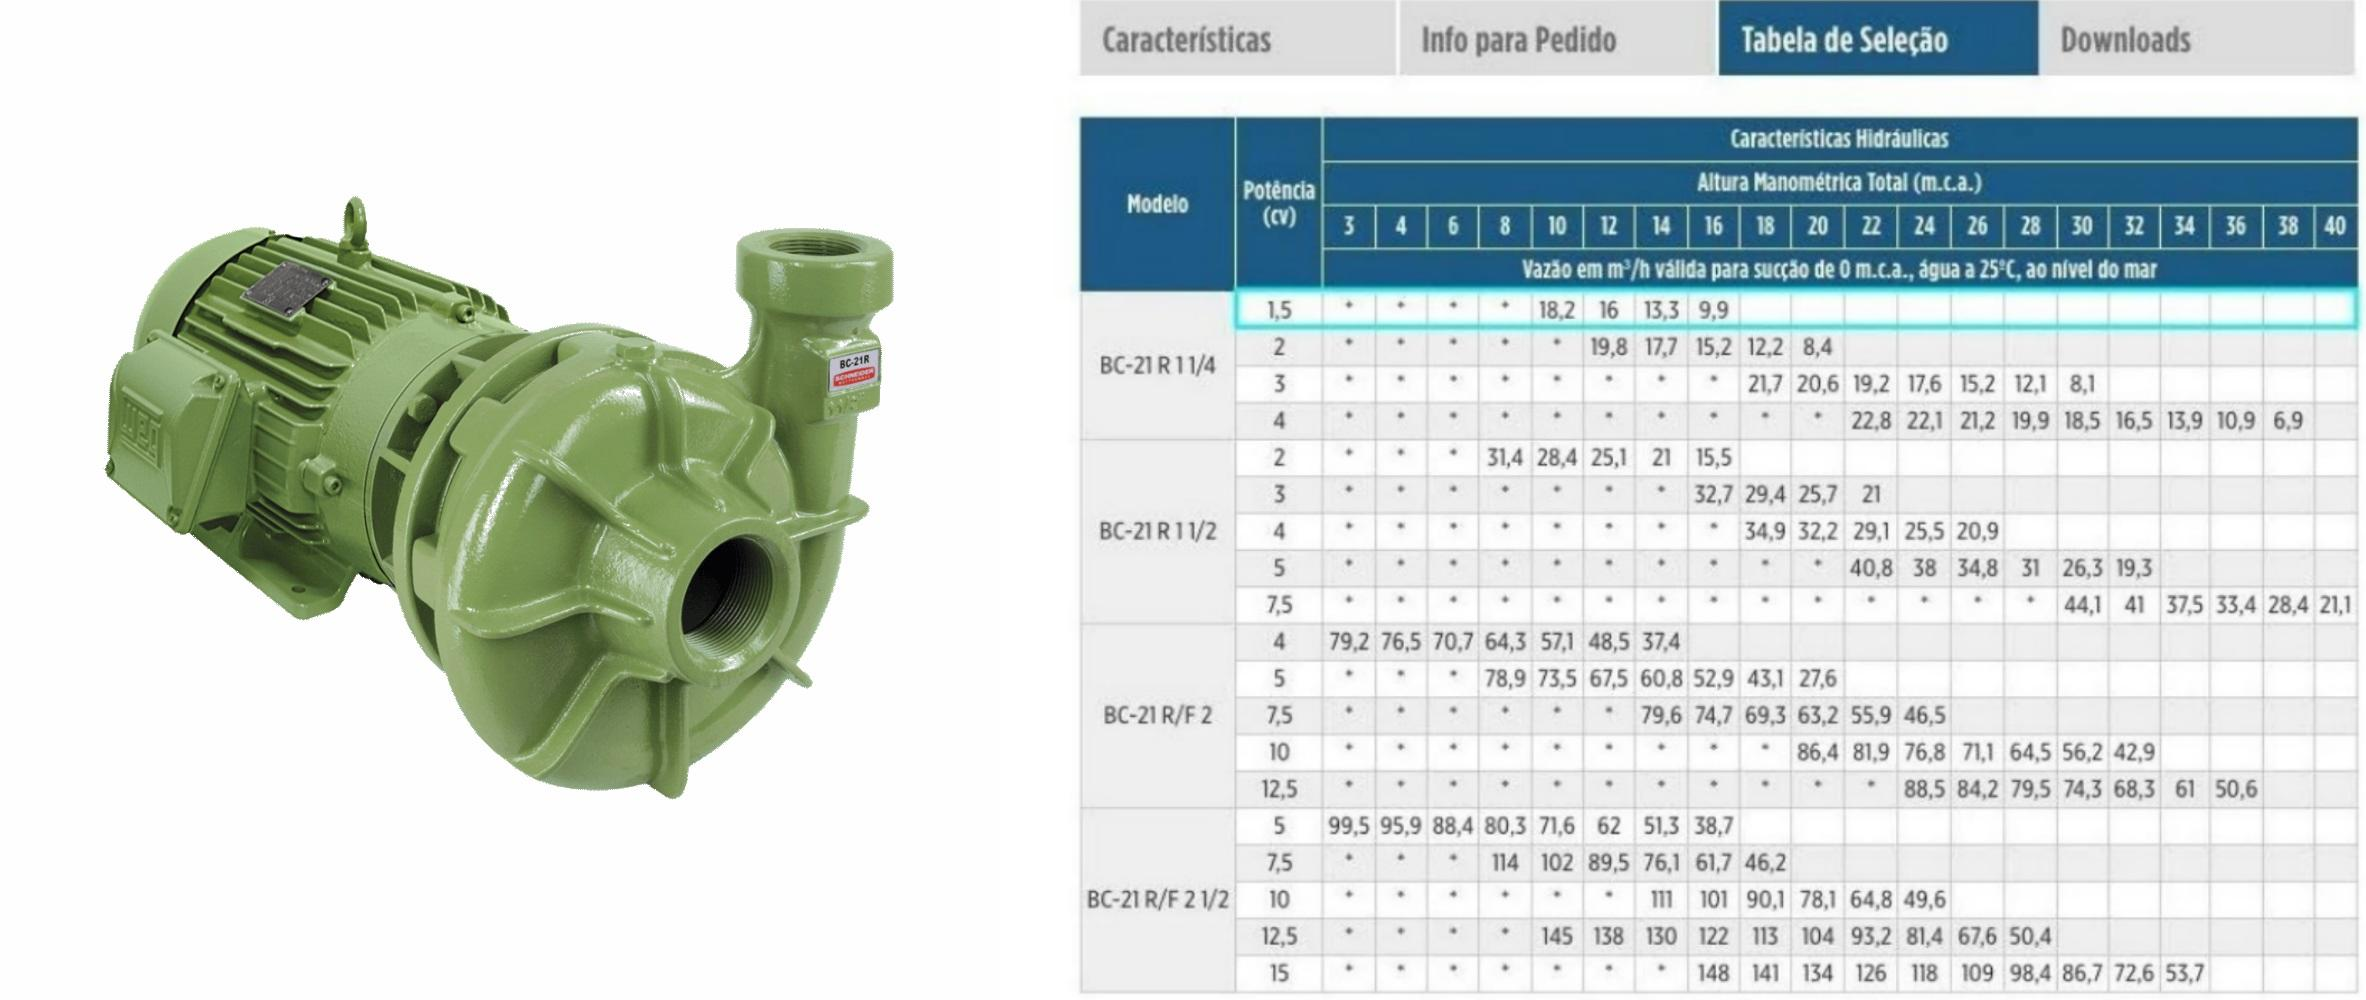
\includegraphics[scale=0.8]{figuras/1111111111111111111111111.jpg}
    \caption{Bomba Modelo - Schneider BC-21 R 1 1/4}
        \label{fig:1}
\end{figure}

\textit{Reservatórios:}

São estruturas que armazenam água para garantir o fornecimento contínuo, mesmo durante períodos de alta demanda ou quando a fonte de água não estiver disponível. Sua capacidade depende da vazão da bomba e da demanda de consumo.

Existem dois tipos principais dessas estruturas. Os reservatórios elevados são geralmente feitos de concreto ou aço e estão elevados do solo para fornecer pressão por gravidade. Já os reservatórios apoiados estão localizados no nível do solo ou enterrados, e requerem bombeamento ou sistemas de pressão para distribuir a água.


No projeto em questão, foi adotado um modelo de reservatório elevado com capacidade máxima de 20 m³. Este modelo foi escolhido por fornecer abastecimento por gravidade, eliminando os gastos com distribuição de água.

\textit{Rede de Distribuição:}

É o sistema de tubulações que transporta a água dos reservatórios até os consumidores. Ela é composta por tubulações principais, secundárias e ramais. A manutenção regular desta rede é crucial para prevenir vazamentos e garantir a qualidade da água.

    
\section{Tarifação e Políticas de Consumo}

A tarifação e as políticas de consumo desempenham um papel decisivo na gestão eficiente dos sistemas de abastecimento de água. São instrumentos que influenciam o comportamento do consumidor e a operação do sistema, visando alcançar objetivos específicos, como a sustentabilidade financeira, a equidade no acesso e o uso racional da água \cite{sancho19WaterConsumption}. 

\subsection*{Tarifação}   

As tarifas podem ser estruturadas de diversas formas, dependendo dos objetivos a serem alcançados, tais como: 

\begin{itemize}

    \item[-] Tarifas Fixas: Um valor fixo é cobrado, independentemente do volume de água consumido. Este tipo de tarifa é simples, mas não incentiva o uso eficiente da água. 

    \item[-] Tarifas Variáveis: A tarifa é baseada no volume de água consumido. Pode ser uma taxa uniforme por unidade de volume ou pode variar de acordo com faixas de consumo, incentivando a economia de água. 

    \item[-] Tarifas Diferenciadas por Horário: As tarifas variam de acordo com o horário do dia, refletindo os custos variáveis de fornecimento. Por exemplo, tarifas mais altas podem ser aplicadas durante os horários de pico, para desencorajar o uso excessivo e aliviar a pressão sobre o sistema.

\end{itemize}


Esquemas tarifários são uma ótima alternativa para a otimização do consumo de energia, pois permitem que decisões sejam tomadas com base nos custos associados a cada tarifa. Por exemplo, pode ser mais econômico operar equipamentos que consomem muita energia durante os períodos em que a tarifa mais barata é aplicada ou evitar consumos excessivos em horários de alta tarifa. 


\subsection{Políticas de Consumo}

Além da tarifação, políticas de utilização podem ser implementadas para gerenciar o consumo de água: 

\begin{itemize}

\item[-] Restrições de Uso: Em situações de escassez, podem ser impostas restrições sobre certos usos não essenciais da água, como rega de jardins ou lavagem de carros. 

\item[-] Programas de Educação: Campanhas de conscientização podem ser lançadas para informar e alertar a população sobre a importância do consumo sustentável de água e energia.

\item[-] Incentivos: Incentivos podem ser oferecidos à população para encorajar práticas de economia de água, como a instalação de dispositivos de baixo fluxo ou a coleta de água da chuva. 

\end{itemize}

No trabalho, foi observado que a tarifação desempenha um papel significativo na otimização do custo de energia associado ao abastecimento de água. Elas são diferenciadas por períodos tarifários, e a operação da bomba é ajustada de acordo com essas tarifas para minimizar os custos. Além disso, políticas fixas com restrições de tarifa de ponta são implementadas para otimizar ainda mais o funcionamento da bomba e os custos associados. 

Essa combinação proporcionou uma otimização no consumo, que pode incentivar uma gestão mais eficiente dos recursos energéticos, beneficiando tanto os prestadores de serviços quanto os consumidores. 

\section{Análise e Visualização dos Dados}
  

\section{Modelagem Matemática}

O problema consistia em determinar o melhor momento para ligar e desligar uma bomba de água, responsável pelo abastecimento de um reservatório, de forma a minimizar os custos com energia elétrica associados, mantendo o nível de água armazenada dentro de limites aceitáveis.

Os custos variam conforme uma tarifa, que muda ao longo do dia e da semana, enquanto o nível do reservatório é determinado pela vazão da bomba, pela demanda de consumo e pela capacidade do próprio reservatório.

O modelo foi formulado como um problema de programação linear inteira mista, usando variáveis binárias para representar o estado da bomba (ligada ou desligada) e variáveis contínuas para representar os níveis do reservatório.

A função objetivo foi projetada para minimizar o custo total com energia elétrica ao longo do horizonte de planejamento de uma semana, sujeita a restrições que incluíam o balanço de massa do reservatório, os limites do nível do reservatório e a relação entre o estado e a vazão da bomba.

\subsection{Formulação matemática}


\subsection{Conjuntos e parâmetros}

\begin{itemize}

\item[-] $h = \left\{1, ..., 24\right\}$: conjunto das horas do dia.

\item[-] $d = \left\{1, ..., 7\right\}$: conjunto dos dias da semana.

\item[-] $C_{h,d}$: custo da energia elétrica na hora $h$ e no dia $d$ ($R\$/kWh$).

\item[-] $P$: potência da bomba ($kW$).

\item[-] $Q$: vazão da bomba ($m^3/h$).

\item[-] $V_{min}$: limite mínimo do nível do reservatório ($m^3$).

\item[-] $V_{max}$: limite máximo do nível do reservatório ($m^3$).

\item[-] $V_{0}$: nível inicial do reservatório ($m^3$).

\item[-] $D_{h,d}$: demanda de consumo na hora $h$ e no dia $d$ ($m^3/h$).

\end{itemize}


\subsection{Variáveis de decisão}

\begin{itemize}

\item[-] $x_{h,d} \in {0, 1}$: variável binária que indica se a bomba está ligada (1) ou desligada (0) na hora h e no dia d.

\item[-] $V_{h,d} \geq 0$: variável contínua que representa o nível do reservatório na hora h e no dia d ($m^3$).
\end{itemize}

\subsection{Função objetivo}

O objetivo é minimizar o custo total com energia elétrica ao longo do horizonte de planejamento, dado por:

$$min \sum_{h=1}^{24} \sum_{d=1}^{7} C_{h,d} P x_{h,d}$$

\subsection{Restrições}

Balanço de massa do reservatório:

\BlankLine

$V_{h,d} = V_{h-1,d} + Q x_{h,d} - D_{h,d}, \forall h \in {2, ..., 24}, \forall d \in D$

$V_{1,d} = V_{24,d-1} + Q x_{1,d} - D_{1,d}, \forall d \in {2, ..., 7}$

$V_{1,1} = V_0 + Q x_{1,1} - D_{1,1}$

\BlankLine

Limites do nível do reservatório:

\BlankLine

 $V_{min} \leq V_{h,d} \leq V_{max}, \forall h \in H, \forall d \in D$


\section{Otimização do Problema}

A otimização da gestão em sistemas de abastecimento de água constitui um desafio multidimensional, que envolve a sincronização entre demanda, oferta e custos operacionais. No presente estudo, abordamos a otimização do funcionamento de bombas de água em um sistema de abastecimento, focando no equilíbrio entre a demanda horária de consumo de água e as variações tarifárias de energia elétrica, com o intuito de minimizar o custo energético sem comprometer a disponibilidade hídrica para os consumidores.

A análise foi iniciada com a criação de uma matriz de demanda horária média, de consumo de água para cada dia da semana, baseada em registros históricos. Cada célula da matriz 
Para a otimização, foram definidos parâmetros críticos, como a potência da bomba, a taxa de fluxo de água e a capacidade do reservatório. O volume inicial do reservatório foi estabelecido, assim como os volumes mínimo e máximo, para assegurar uma operação dentro dos limites seguros e eficientes.


\subsection{Estratégia de Tarifação Dinâmica}

A estratégia de tarifação dinâmica foi implementada considerando três tarifas distintas, baseadas na bandeira verde: a tarifa vermelha, para horários de pico; a tarifa amarela, para horários intermediários; e a tarifa verde, para horários de baixa demanda. A função de precificação foi configurada para atribuir a tarifa correspondente a cada intervalo horário, com diferenciação entre dias úteis e fins de semana.


\subsection{Algoritmo de Simulação de Operação das Bombas}


\subsection{Monitoramento e Restrições de Operação}

As restrições de operação, como níveis críticos do reservatório e a capacidade máxima de bombeamento, foram rigorosamente monitoradas, e qualquer violação das restrições foi registrada para posterior análise e ajuste da estratégia de operação.


Visualizações gráficas foram criadas para ilustrar o consumo de água por hora e dia da semana, o nível do reservatório ao longo do tempo, o custo acumulado da energia elétrica e a distribuição temporal da operação das bombas em relação às tarifas aplicadas. Essas visualizações foram fundamentais para identificar padrões de consumo, avaliar a eficácia das estratégias de operação e compreender o impacto das tarifas na operação do sistema.



\subsection{Conclusão}

Ao final do processo de otimização, observou-se uma redução significativa nos custos com energia elétrica, indicando a eficiência das estratégias de operação adotadas. Com a primeira política de funcionamento, sem restrição de funcionamento em horários de pico, o consumo semanal foi de R\$ 12,97, enquanto que com a política proposta, restritiva quanto ao funcionamento das bombas em horário de pico o custo foi de R\$ 8,71, uma economia de 32.85\%.

Portanto, a abordagem implementada demonstrou ser uma solução viável para a gestão sustentável de sistemas de abastecimento de água, equilibrando custos operacionais e disponibilidade hídrica.

	\chapter{Resultados e Discussões}
\label{chap:resultados}


	\chapter{Conclusões e Implementações Futuras}
\label{chap:conclusoes}

O modelo atual de otimização é projetado para melhorar a gestão do sistema de abastecimento de água. Contudo, a adição de novos elementos ao modelo pode enriquecê-lo e gerar resultados mais significativos. Uma proposta é a expansão da estratégia tarifária, que envolve a ampliação do modelo para incorporar uma abordagem mais detalhada das tarifas energéticas, que frequentemente variam em horários não-inteiros. Além disso, o modelo pode ser aprimorado para refletir diferentes bandeiras tarifárias. O resultado esperado dessa expansão é uma maior flexibilidade e precisão na gestão de custos, permitindo a adaptação das operações de bombeamento a um espectro mais amplo de condições tarifárias e alinhando a gestão de custos com as variações reais do mercado.

Outro aspecto crucial é a realização de uma análise de sensibilidade aprimorada. Para isso, a aplicação do Método de Monte Carlo pode ser explorada para avaliar o impacto de variações estocásticas nos custos de energia, padrões de consumo e outras variáveis operacionais. Este método permite simular diversos cenários, proporcionando uma visão mais clara das incertezas e riscos associados. O resultado esperado desta análise é a identificação de pontos críticos do sistema e uma capacidade aprimorada de prever e gerenciar riscos operacionais, oferecendo insights valiosos para o sistema em condições adversas.

Adicionalmente, a aplicação de outras técnicas de otimização é recomendada. Isso inclui a implementação de métodos como otimização estocástica, metaheurísticas ou novas políticas de gestão de consumo, para avaliar o desempenho do sistema. O resultado esperado dessas técnicas é um aumento na robustez do modelo, tornando-o mais resiliente a incertezas e variações no consumo e fornecimento de água.

Por fim, a expansão do conjunto de dados utilizado no modelo é fundamental. Enriquecer o modelo com dados mais abrangentes, incluindo séries temporais mais extensas, dados demográficos e informações econômicas, pode proporcionar uma compreensão mais profunda das tendências de longo prazo e das influências econômicas no consumo de água. O resultado esperado dessa expansão é a capacidade de realizar previsões e planejamentos mais precisos.
	
	%Elementos pós-textuais	
	\bibliography{3-pos-textuais/referencias}
%	\imprimirglossario 	
%	\imprimirapendices 
		% Adicione aqui os apendices do seu trabalho
		%\input{3-pos-textuais/apendices/apendice-a}
		%\input{3-pos-textuais/apendices/apendice-b}
		%\input{3-pos-textuais/apendices/apendice-c}
		
%		\imprimiranexos
		% Adicione aqui os anexos do seu trabalho
		%\input{3-pos-textuais/anexos/anexo-a}
		%\input{3-pos-textuais/anexos/anexo-b}		
    %\imprimirindice
    
	

\end{document}